\documentclass[parskip=full]{scrartcl}
\usepackage[utf8]{inputenc} % use utf8 file encoding for TeX sources
\usepackage[T1]{fontenc}    % avoid garbled Unicode text in pdf
\usepackage[english]{babel}  % english hyphenation, quotes, etc
\usepackage{hyperref}       % detailed hyperlink/pdf configuration
\hypersetup{                % ‘texdoc hyperref‘ for options
pdftitle={HePICS Design Document},%
bookmarks=true,%
}
\usepackage{graphicx}       % provides commands for including figures
\usepackage{csquotes}       % provides \enquote{} macro for "quotes"
\usepackage{enumitem}


\title{HePICS Design Document}

\begin{document}

\maketitle
\thispagestyle{empty}
\pagebreak





\tableofcontents
\pagebreak





\section {Functionality Description}

In the model part, classes realize the management of all the data and logic. They load pathes of input images and access their features. The classification results are stored in the type of string to be shown in various forms. The logic of classification is determined by the neural network being used. Its topology defines how different layers interact with each other. With the assistance of all the layers, the forward propagation functionality can be implemented, which is the core of algorithms for image classification with pre-trained model.

The view realizes the user interfaces. The welcome window and the main window, which contains three different sections, guide the user to upload his input files, select available platforms and operating mode, let him control the process and show the prediction results. 

The controller accepts user inputs handled by the components of the views and converts them to the commands. The classifier controls the progress of processing and assigns the scheduler to dispatch work to workers in heterogeneous platforms. In addition, the poller checks the requests from external systems regularly. After receiving the correct request with the image path, the classifier starts the process of classification.



\section {Class Diagram Description}

In this diagram several design patterns were used.
In order to decouple  major components and allow parallel development we use the Model-View-Controller as a global architecture.
The class diagram consists of several common patterns to reduce complexity and dependencies between classes.
We use the template Method as pattern for sections to define the skeleton of the algorithm in an operation.
However the results and states are updated using an observer which defines a one-to-many dependency between objects.
Different Modes as well as Worker are represented by simple is-relationships.
Another interesting pattern to be used by layers is the strategy-pattern. In this context we define a family of algorithm, encapsulate
each one and make them interchangeable. This approach also lets the algorithm vary independently from the layer that uses it.

\pagebreak

\section {Class Description}

\begin{itemize}
	\item HepicsGui: represents the main entry point to execute the software. It contains the main Method.
	\item WelcomeWindow: This class is used to display informations about the developed software.
	\item MainWindow: is the main class that runs the classification system. It is also responsable for setting up the GUI.
	\item Section: creates a label for each part of the GUI. It has the template method addLabel() which will be implemented by the different sections. Suclasses define sections (e.g. buttons, check boxes) and handle their actions.
	\item ImageSection: allows the user to add and delete input images. This sections consists of a one combo box which lists all chosen images, three buttons and a thumbnail image.
	\item Plattform\_Mode\_Section: allows the user to choose operation mode and a platform to run the classification or aggregation on it. A checkbox allows the user to choose one or more plattform and a combo box is used to select the mode.
	\item ControlSection: allows the user to start, pause, resume and cancel the classification process. Thus three buttons are used in this context
	\begin{itemize}
		\item Once the classification starts, the start button becomes a cancel button. 
		\item While running the user can pause the classification by clicking on the pause button. 
		\item When paused the pause button becomes a resume button.
	\end{itemize}
	\item Observer: defines an updating interface for objects that should be notified of changes in a subject.
	\item ObserverManager: provides an interface for attaching and detaching Observer objects. It notifies concrete observers whenever corresponding data changes.
\end{itemize}



\pagebreak



\begin{itemize}
	\item ResultObserver, StateObserver: implement the Observer updating interface to keep its state consistent with concrete subjects and maintain reference to those subjects. These observers might be considered respectively as result section and state section:
	\begin{itemize}
		\item The result section contains results of aggregation. The results are represented in form of text. The results are the probabilities of the top detected objects in percentages.
		\item The state section is mainly the progress bar which shows the state of the current running process.
	\end{itemize}
	\item Class-Image: is an abstract class which represents the modelisation of an image in the programming language. Its attributes are length, width, channel, and id, which means each uploaded or created image is unique. This class is only a representation of an image object, it can be replaced by an existing library.
	\begin{itemize}
		\item Attributes:
		\begin{itemize}
			\item length: is the length of the image object
			\item width: is the width of the image object
			\item channel: number of channels of the image, by default set to 3 (Red, Green, Blue)
			\item id: is a unique number for each image, used to identify them and differentiate them from each other.
		\end{itemize}
		\item Methods:
		\begin{itemize}
			\item getLength(): returns the length of the image	
			\item setLength(length:int): sets the value of the image's length	
			\item getWidth(): returns the width of the image
			\item setWidth(width:int): sets the value of the image's width
			\item getChannel(): returns the number of channels the image has
			\item setChannel(channel:int): sets the number of channels of the image
			\item resize(length : int, width : int): changes the size of the image to the new dimensions
		\end{itemize}
	\end{itemize}
\end{itemize}



\pagebreak



\begin{itemize}
	\item Class-InputImage: represents an input image. Has an extra attribute isClassified, which tells if the image has already been classified. In this case, it is not necessary to redo the classification. It is also possible to create a thumbnail out of this image.
	\begin{itemize}
		\item Attributes: 
		\begin{itemize}
			\item isClassified : a boolean which tells if the image has already been classified. True : display results without classifying, false : start a normal classification process.
		\end{itemize}
		\item Methods:
		\begin{itemize}
			\item createThumbnail() : creates a thumbnail of the input image and returns it as an image. A thumbnail is a smaller representation of the image itself.
			\item setStatus( b : boolean) : changes the status of the image to classified or non classified.
			\item getStatus() : returns the status of the image : classified/true, not classified/false
		\end{itemize}
	\end{itemize}

	\item Class-ResultImage : represents the image that is displayed which contains the results of the classification. It has an extra attribute called result, which is a string containing the results. These results can also be displayed in other ways if it is wished to extend the functionality of the system (histograms, pie charts)
	\begin{itemize}
		\item Attributes:
		\begin{itemize}
			\item result : a string which contains the results of the classification of an image in percentages.
		\end{itemize}
		\item Methods:
		\begin{itemize}
			\item getResult() : returns the string containing the results of the classification.
			\item setResult( results: String) : sets the results of a classification
			\item createResult() : draws the results of a classification contained in the string on an image and returns it. This method can be later modified in such way that results would be displayed in a better way.
		\end{itemize}
	\end{itemize}
\end{itemize}



\pagebreak



\begin{itemize}
	\item Class-ImageManager : is responsible for providing the input image to the system and its preprocessing, which means, converting it into a matrix, or an RGB image, depending on what the process needs.
	\begin{itemize}
		\item Attributes:
		\begin{itemize}
			\item input  : is the image object representation of the input image.
			\item inputPath : is a String which contains the path to the input image
		\end{itemize}
		\item Methods:
		\begin{itemize}
			\item getPath() : returns a string containing the path to the input image
			\item setPath( path : String) : sets the path of the input image
			\item loadInput(path  : String ) : loads the input image from its path and returns it
			\item convertRGB(input : Image, length : int, width : int, channel : int) : returns an RGB image of the input image for the sake of the classification.
			\item preProcessImage : returns the image in the form of a matrix for the sake of the classification.
			\item getImage() : returns the input image.
		\end{itemize}
	\end{itemize}
\end{itemize}



\pagebreak



\begin{itemize}
	\item Class-DataSaver : is practically the data holder. It saves the input images loaded during the time the system has been running in a hashmap. Can also write the results in a text file, and aggregate the results of the given inputs. Aggregating results means in this case calculating the average of multiple results for the corresponding input images. The goal behind it is to achieve higher precision in the classification through selecting more than one image of the same object for the classification.
	\begin{itemize}
		\item Attributes:
		\begin{itemize}
			\item results : is a hashmap whose key is the id of the images, and value is the results of the classification of the corresponding image.
		\end{itemize}
		\item Methods:
		\begin{itemize}
			\item addResult( input : InputImage, result :  ResultImage) : adds the result of the classification of an input image
			\item setResult( input : InputImage, result : ResultImage) : sets the result of the classification of an input image
			\item getResult( input : InputImage) : returns the result of the classification of an input image 
			\item aggregate() : aggregates the results of the last classification process, if there are multiple inputs  
			\item writeFile( id : int) : writes the results of the corresponding input image to a text file 
		\end{itemize}
	\end{itemize}
\end{itemize}



\pagebreak



\begin{itemize}
	\item Class-ClassificationAssistant : is practically the classifier's secretary. It makes sure that the classifier gets all what it needs to run the classification. It loads weights, sets the input image in the wished form, and loads all the neural networks needed specifications, as well as the classification's class names. Input images get transfered one by one through the assistant.
	\begin{itemize}
		\item Attributes:
		\begin{itemize}
			\item inputImage : is the input image
			\item weightFilePath : is a String containing the path to the weights file.
			\item weights : is an array of double containing the weights of the neural network
			\item classNamesPath : is a string containing the path to the class names file. These are the objects to be identified during the classification.
			\item isClassified() : is a boolean which tells if the currently loaded input image is classified. By default, it is set on false.
			\item manager : is an instance of the class ImageManager. It is responsible for the necessary preprocessing of the input image.
		\end{itemize}
		\item Methods:
		\begin{itemize}
			\item getNeuralNetwork() : returns the currently established neural network
			\item setNeuralNetwork( nn : NeuralNetwork) : sets the currently established neural network
			\item getInputImage() : returns the currently loaded input image
			\item setWeights( weights : Array of double) : sets the array of weights through a new one
			\item getWeights() : returns an array of double which contains the weights of the neural network
			\item loadClassNames() : returns an array of string containing the class names.
			\item getClassNamesPath() : returns a string containing the path to the class names file
			\item setClassNamesPath( path : String ) : sets the path to the class names file
		\end{itemize}
	\end{itemize}
\end{itemize}



\pagebreak



\begin{itemize}
	\item Class-NeuralNetwork : is the modelisation of a neural network. A neural network has a name, a topology and a set of layers.
	\begin{itemize}
		\item Attributes:
		\begin{itemize}
			\item name : a string containing the name of the neural network
			\item topology : an instance of the class topology. It is a characteristic of the neural network
			\item layers : is an array of layers that build the neural network
		\end{itemize}
		\item Methods:
		\begin{itemize}
			\item getName() : returns the name of the neural network
			\item setName( name : String) : sets the name of the neural network
			\item getTopology() : returns the topology object of the neural network
			\item setTopology( topology : Topology) : sets the topology of the neural network through a new one
			\item addLayer( type : LayerType) : adds a layer to the list of layers of the neural network
			\item forwardPropagation ( inputImage : Image) : returns a matrix of floats that represent the build through the classification.
		\end{itemize}
	\end{itemize}
\end{itemize}



\pagebreak



\begin{itemize}
	\item Class-Shape : contains constants which define the dimensions, which means the form and general composition of a layer represented as a matrix.
	\begin{itemize}
		\item Attributes:
		\begin{itemize}
			\item rows : the number of rows of the layer and the first dimension of the matrix
			\item cols : the number of columns of the layer and the second dimension of the matrix
			\item channels : the number of channels of the layer and the third dimension of the matrix
		\end{itemize}
		\item Methods:
		\begin{itemize}
			\item getRow() : returns the number of rows of the layer
			\item getCols() : returns the number of columns of the layer
			\item getChannels() : returns the number of channels of the layer
		\end{itemize}
	\end{itemize}


	\item Class-Topology : is the visual representation of the neural network, meaning the layers and the relations or interactions between them.
	\begin{itemize}
		\item Attributes:
		\begin{itemize}
			\item displayer : is an instance of the class TopologyDisplayer.
		\end{itemize}
		\item Methods:
		\begin{itemize}
			\item display() : displays the topology of the neural network.
		\end{itemize}
	\end{itemize}
\end{itemize}



\pagebreak



\begin{itemize}
	\item Class-TopologyDisplayer : is a tool which is responsible for drawing the representation of the topology and generating an image.
	\begin{itemize}
		\item Attributes:
		\begin{itemize}
			\item layers : is a list of the layers that constitute the neural network
			\item display : is an image on which the topology is drawn
		\end{itemize}
		\item Methods:
		\begin{itemize}
			\item drawTopology() : draws the topology on an image and returns it
			\item getDisplay() : returns the image to display
		\end{itemize}
	\end{itemize}


	\item Class-Layer : is what a neural network is made of. It is a set of nodes placed on each other which each treat the input image depending on their type and activation function.
	\begin{itemize}
		\item Attributes:
		\begin{itemize}
			\item type : is an enumeration called LayerType. It defines the type of the layer, and on that note, the way it handles the treatment of the data it receives.
		\end{itemize}
		\item Methods:
		\begin{itemize}
			\item getType() : returns the type of the layer.
			\item setType( type : LayerType) : sets the type of the layer
			\item getInputShape() : returns the shape of the input
			\item setInputShape() : sets the shape of the input
			\item getOutputShape() : returns the output's shape
			\item setOutputShape() : sets the shape ouf the ouput
			\item forwardPropagation(inputImage : Image) consists of processing the data of the input image through one layer, it returns a matrix of float values
		\end{itemize}
	\end{itemize}
\end{itemize}



\pagebreak



\begin{itemize}
	\item Enumeration Class-LayerType : is an enumeration class of the possible layer types. Each type defines how the layer treats the data it receives and how it gives it over to the next one.
	\begin{itemize}
		\item InputLayer
		\item ConvolutionalLayer
		\item MaxPoolLayer
		\item ResponseNormalizationLayer
		\item DenseLayer
		\item FullyConnectedLayer
	\end{itemize}
	\item InputLayer Class: This class inherits the abstract Layer class. It is the first layer of a neural network model, which contains the input shape of an input image as its attribute.
	\item Abstract ConvolutionalLayer Class: This class modifies the convolutional layers, which applies a specified number of convolution filters to the image. For each subregion, the layer performs a set of mathematical operations to produce a single value in the output feature map. 
The filters attribute specifies the number of filters to apply, kernel\_size specifies the dimensions of the filters and strides specifies the strides of the convolution along the height and width.
	\item CPUConvolutionalLayer Class: This class inherits the abstract ConvolutionalLayer Class. Its computation would be executed on the CPU. 
	\item FPGAConvolutionalLayer Class: This class inherits the abstract ConvolutionalLayer Class. Its computation would be executed on the FPGA. 
\end{itemize}



\pagebreak



\begin{itemize}
	\item MaxPoolLayer Class: This class modifies the maxpool layer, which downsample the image data extracted by the convolutional layers to reduce the dimensionality of the feature map in order to decrease processing time. It uses max pooling as its pooling algorithms, which extracts subregions of the feature map (e.g., 2x2-pixel tiles), keeps their maximum value, and discards all other values.
The pool\_size attribute specifies the size of the max pooling filter as [height, width]. If both dimensions have the same value, you can instead specify a single integer and the strides specifies the size of the stride.
	\item ResponseNormalizationLayer Class: This class modifies the response normalization layer, which normalizes the activations of the previous layer at each batch, i.e. applies a transformation that maintains the mean activation close to 0 and the activation standard deviation close to 1. The axis attribute specifies the axis that should be normalized (typically the features axis).
	\item DenseLayer Class: This class modifies the dense layer, which performs classification on the features extracted by the convolutional layers and downsampled by the pooling layers. In a dense layer, every node in the layer is connected to every node in the preceding layer.
The units attribute specifies the number of neurons in the dense layer.
	\item TrainableLayer Class: This class modifies the layer whose trainable parameters (e.g. weights) can be optimized and updated by the training algorithms (like back-propagation). The weight attribute specifies the weights of this layer and use\_bias specifies whether the layer uses a bias vector. The getWeight method returns the weights of the layer as a matrix and setWeight method sets the weights of the layer from a matrix (with the same shapes as the output of getWeight). All the layers implement the forward propagation method in order to use the pre-trained parameters to get the output. 
	\item ActivationFunction Class: This abstract class encapsulates the activation function whose purpose is to allow small changes in the weights or bias to only cause a small change on the output, this property is helpful when training a network.
The name attribute specifies the name of the activation function.
The activate method specifies the function that would be applied.
\end{itemize}



\pagebreak



\begin{itemize}
	\item Sigmoid Class: This class encapsulates an activation function called Sigmoid. Its method activate implements the function: $g(z) = 1 / (1 + e^{-z})$. It’s used on the output layer so that we can easily interpret the output as probabilities since it has restricted output between 0 and 1.
	\item Tanh Class: This class encapsulates an activation function called Tanh. Its method activate implements the function: $g(z) = (e^z -e^{-z}) / (e^z + e^{-z})$. It’s superior to sigmoid function in which the mean of its output is very close to zero, which in other words center the output of the activation units around zero and make the range of values very small which means faster.
	\item ReLU Class: This class encapsulates an activation function called ReLU. Its method activate implements the function: $g(z) = max{0, z}$. The models that are close to linear are easy to optimize. Since ReLU shares a lot of the properties of linear functions, it tends to work well on most of the problems.
	\item Softmax Class: This class encapsulates an activation function called Softmax. Its method activate generates a value between 0–1 for each node (the sum of all these softmax values is equal to 1). We can interpret the softmax values for a given image as relative measurements of how likely it is that the image falls into each target class.
	\item ReLU Class:  g(z) = max{0, z}. The models that are close to linear are easy to optimize. Since ReLU shares a lot of the properties of linear functions, it tends to work well on most of the problems.
	\item FileLoader: A dialog used to open files.
	\item LayerType: Defines a constant for every type of layer.
\end{itemize}



\pagebreak



\begin{itemize}
	\item Mode: An interface for classification modes. It has methods for different workers.
	\begin{itemize}
		\item Methods:
		\begin{itemize}
			\item nextFileLoadWorkUnit(): returns the next work unit for a file loading worker
			\item nextCpuWorkUnit(): returns the next work unit for a cpu worker
			\item nextFpgaWorkUnit(): returns the next work unit for a fpga worker
		\end{itemize}
	\end{itemize}
	\item HighPerformanceMode: A class that implements the methods of interface Mode. Its methods are optimized for high performance.
	\item LowPowerMode: A class that implements the methods of interface Mode. Its methods are optimized for low power.
	\item EnergyEfficiencyMode: A class that implements the methods of interface Mode. Its methods are optimized for energy efficiency.
	\item WorkUnit: An interface for units of work.
	\begin{itemize}
		\item Methods:
		\begin{itemize}
			\item run(): runs the unit of work
		\end{itemize}
	\end{itemize}
	\item ImageLoadWorkUnit: Implements a unit of work for loading images.
	\item LayerWorkUnit: Implements a unit of work for calculating a Layer of the neuronal network.
	\item Scheduler: The Scheduler uses the mode to decide which work unit to use next. The mode is set by the respective methods. The Scheduler also holds the RessourceManager. It is able to control the execution and report about its progress.
\end{itemize}



\pagebreak



\begin{itemize}
	\item RessourceManager: Manages ressources for classification. The only ressource at the moment is a counter for files.
	\begin{itemize}
		\item Attributes:
		\begin{itemize}
			\item fileTokens: a counter for file tokens
		\end{itemize}
		\item Methods:
		\begin{itemize}
			\item takeFileToken(): decrements the file token counter and blocks if the counter is 0 (like a semaphore)
			\item returnFileToken(): increments the file token counter
		\end{itemize}
	\end{itemize}
	\item Classifer: Controls the classification. Holds the Workers. It creates and deletes workers based on which platforms are enabled.
	\begin{itemize}
		\item Methods:
		\begin{itemize}
			\item start(): takes the file list and starts the classification
			\item pause(): pauses the classification when running
			\item resume(): resumes the classification when paused
			\item stop(): stops the classification
			\item getProgress(): returns the progress of the classification
			\item enableCpu(): when enabling/disabling the cpu platform cpu  workers are added/removed
			\item enableFpga(): when enabling/disabling the fpga platform fpga  workers are added/removed
			\item enableGpu(): when enabling/disabling the gpu platform gpu  workers are added/removed
			\item addWorker(): adds a new worker to the list
			\item deleteWorker():  deletes a worker to the list
		\end{itemize}
	\end{itemize}
\end{itemize}



\pagebreak



\begin{itemize}
	\item Poller: A class for polling a file. The file gets requests for classification. The class extracts the requests.
	\begin{itemize}
		\item Attributes:
		\begin{itemize}
			\item inputPath: the path to the request file
			\item hasRequest: a boolean that saves if a request has been polled
			\item priority: the priority of the next request
		\end{itemize}
		\item Methods:
		\begin{itemize}
			\item poll(): polls the request file
			\item getHasRequest(): gets if a request has been polled
			\item setHasRequest(): sets if a request has been polled
			\item getPath(): gets the path to the request file
			\item setPath(): sets the path to the request file
			\item getPriority(): gets the priority of the request
			\item setPriority(): sets the priority of the request
		\end{itemize}
	\end{itemize}
\end{itemize}



\pagebreak



\begin{itemize}
	\item Worker: The abstraction of a worker. Uses a thread for execution.
	\begin{itemize}
		\item Attributes:
		\begin{itemize}
			\item t: the thread used for execution
		\end{itemize}
		\item Methods:
		\begin{itemize}
			\item run(): the main loop of the thread
			\item runWorkUnit(): runs the work unit
		\end{itemize}
	\end{itemize}
	\item GpuWorker: A class implementing the worker for GPU usage.
	\item FileLoadWorker: A class implementing the worker for loading files.
	\item CpuWorker: A class implementing the worker for CPU usage.
	\item FpgaWorker: A class implementing the worker for FPGA usage.
\end{itemize}



\pagebreak



\section {Diagrams}

\subsection {Overview Sequence Diagram}

\begin{center}
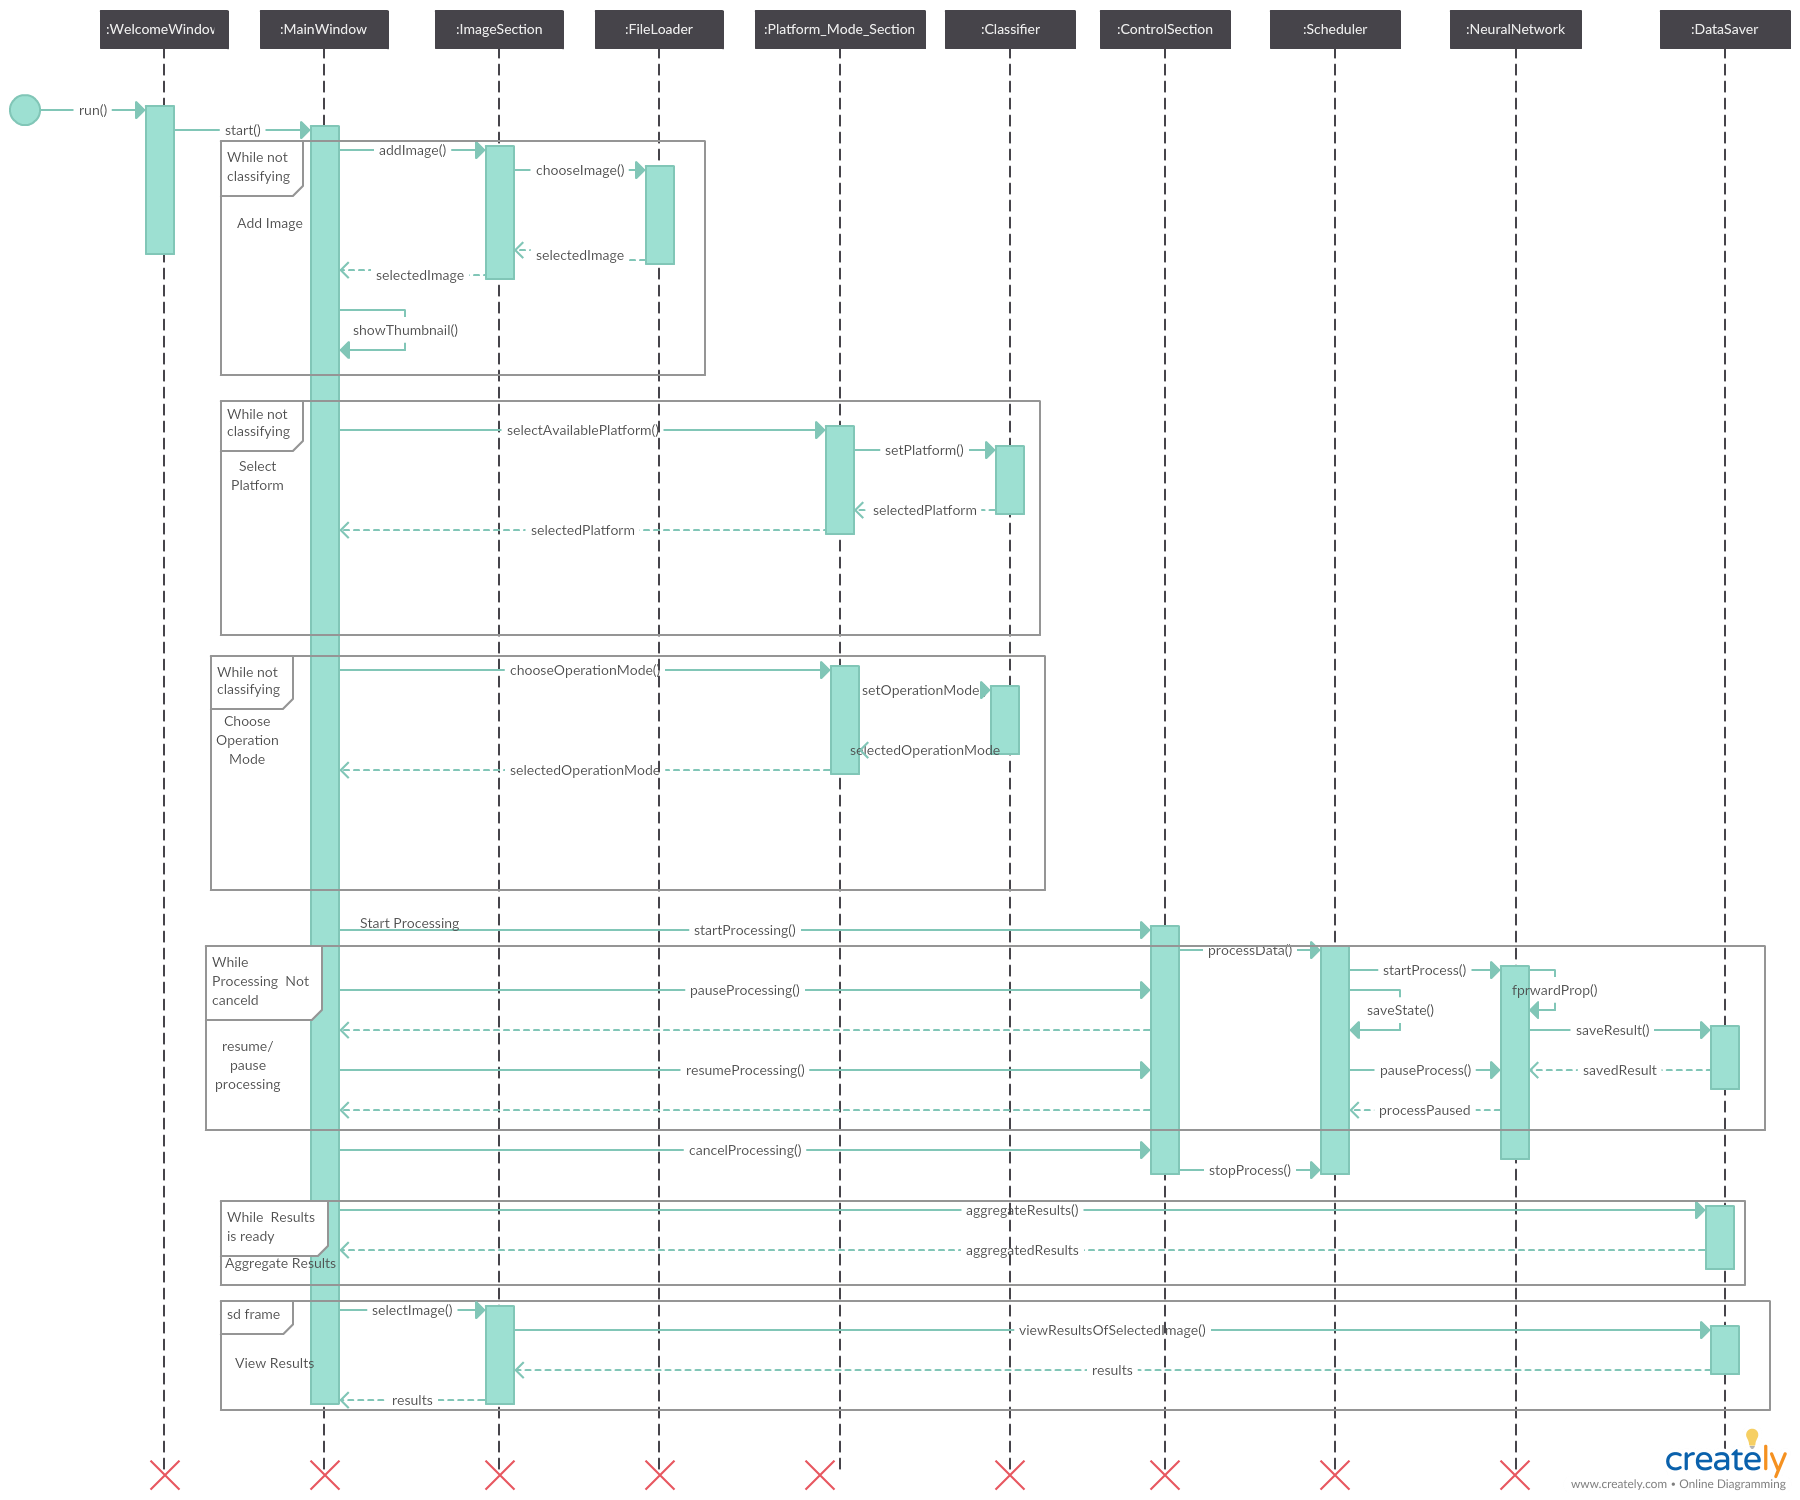
\includegraphics[width=1.0\textwidth]{seq-Diag.png}
\end{center}

\pagebreak

\subsection {Select Platforms Sequence Diagram}

\begin{center}
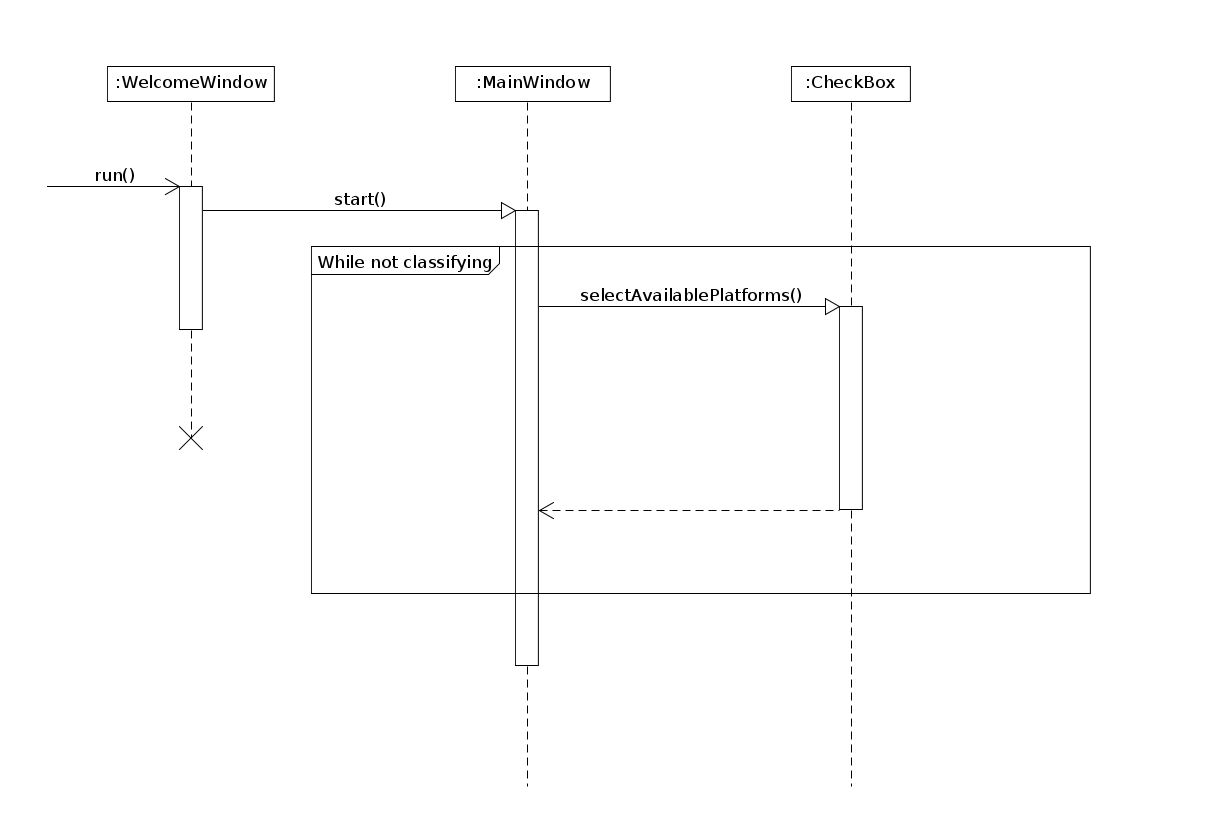
\includegraphics[width=1.0\textwidth]{SelectPlatforms.jpg}
\end{center}

\subsection {Select Image Sequence Diagram}

\begin{center}
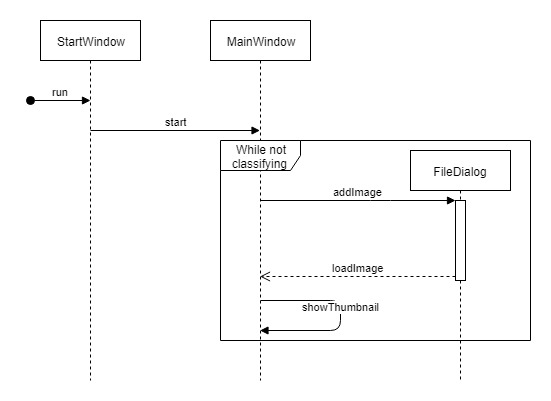
\includegraphics[width=1.0\textwidth]{SelectImageSeqDiag.jpg}
\end{center}

\pagebreak

\subsection {Classification Sequence Diagram}

\begin{center}
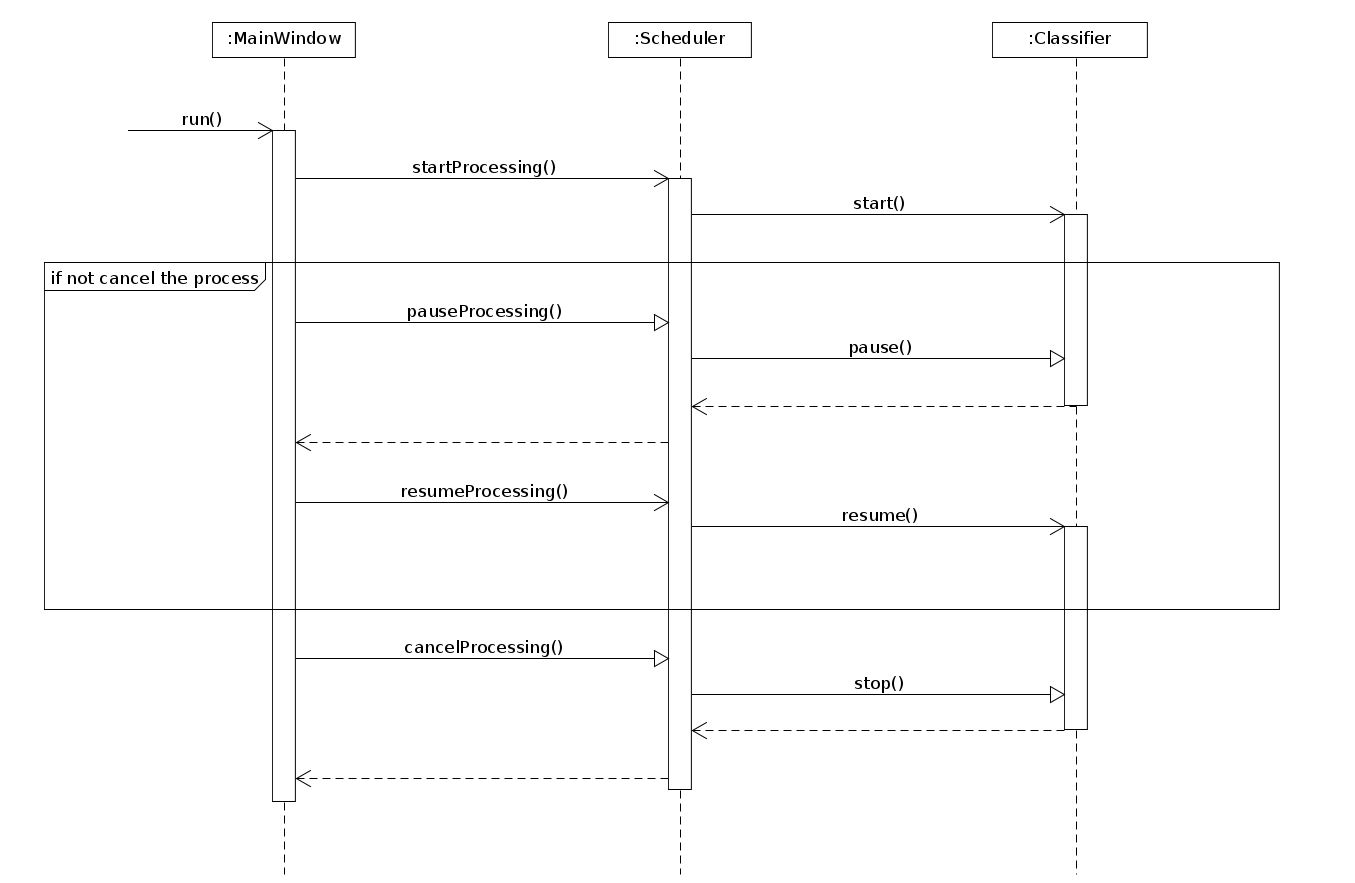
\includegraphics[width=1.0\textwidth]{Classification.jpg}
\end{center}

\pagebreak

\subsection {View Results Sequence Diagram}

\begin{center}
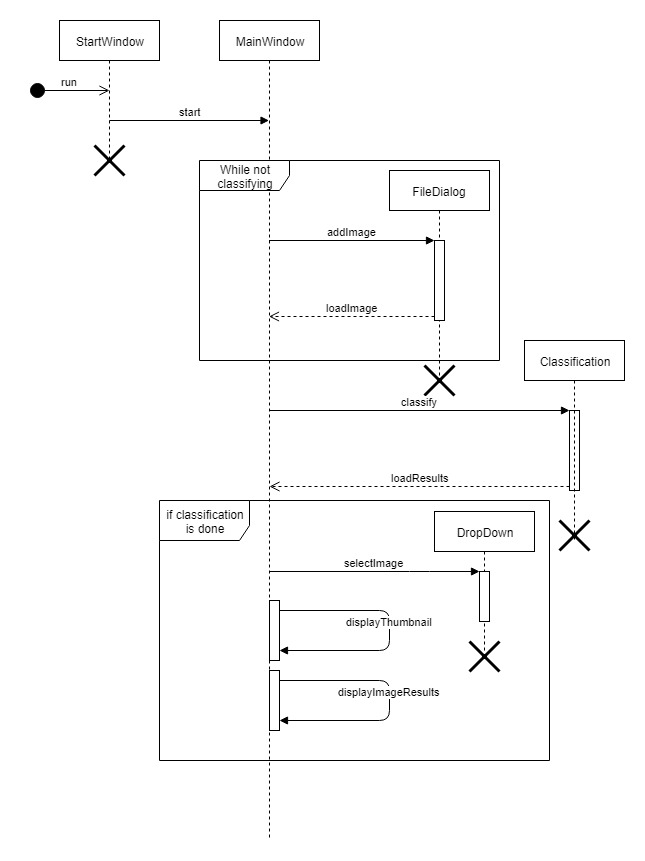
\includegraphics[width=1.0\textwidth]{ViewResults.jpg}
\end{center}

\pagebreak

\subsection {Aggregate Sequence Diagram}

\begin{center}
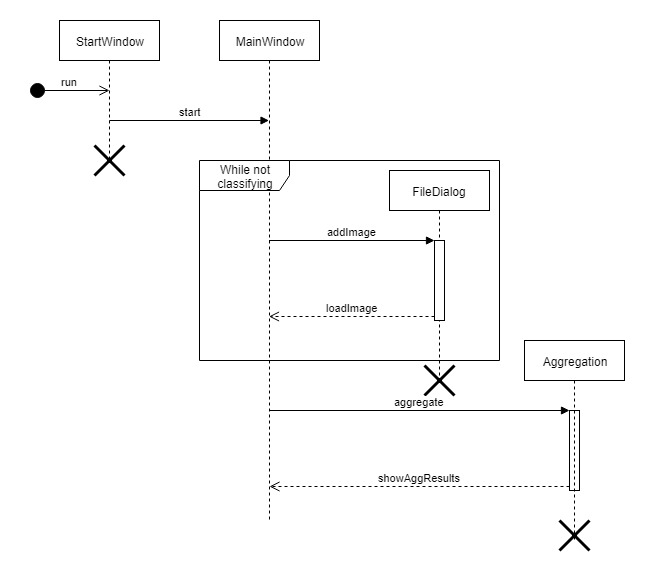
\includegraphics[width=1.0\textwidth]{Aggregate.jpg}
\end{center}

\pagebreak

\subsection {Select Operation Mode Sequence Diagram}

\begin{center}
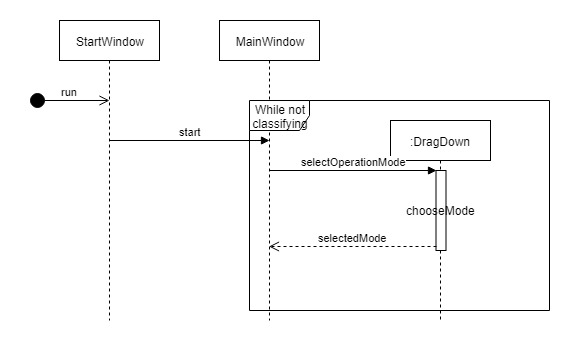
\includegraphics[width=1.0\textwidth]{SelectOperationModeSequenceDiag.jpg}
\end{center}

\pagebreak

\subsection {External Use Sequence Diagram}

\begin{center}
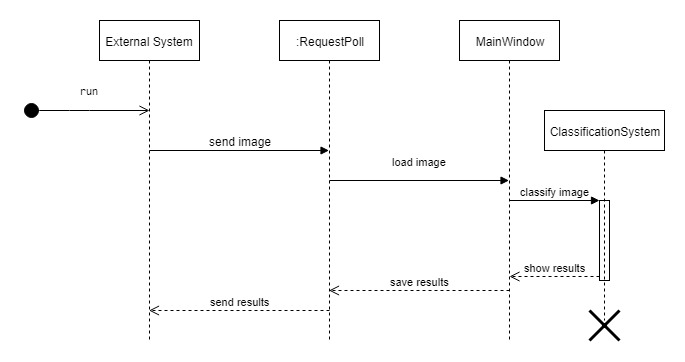
\includegraphics[width=1.0\textwidth]{Untitled Diagram.jpg}
\end{center}

\pagebreak

\subsection {State Diagram}

\begin{center}
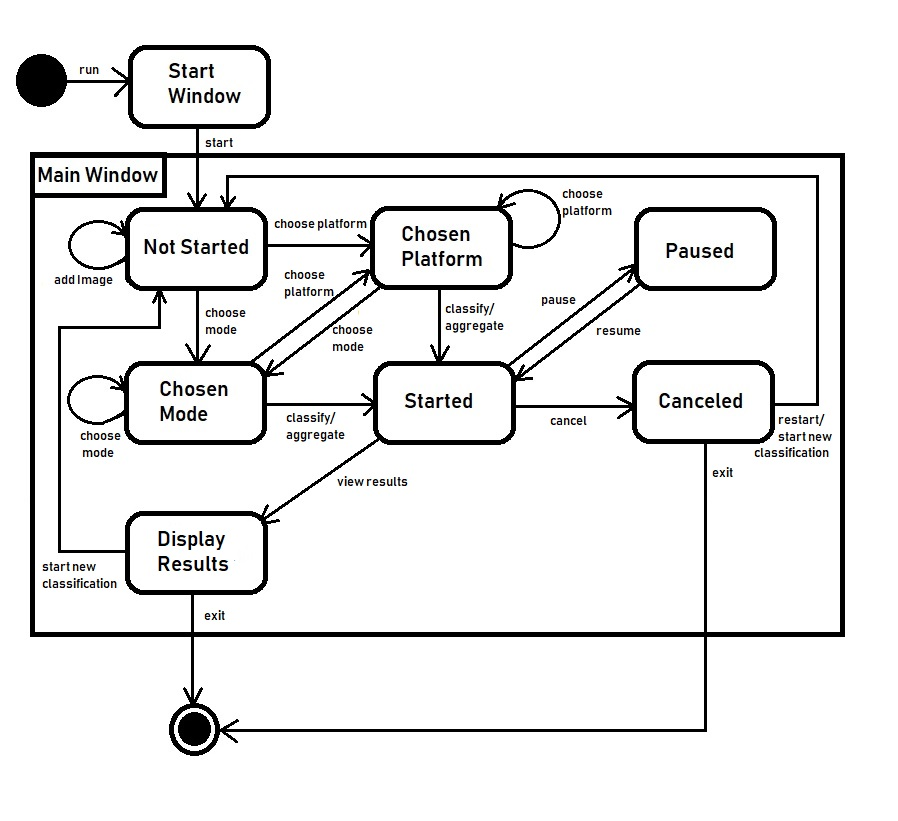
\includegraphics[width=1.0\textwidth]{StateDiag.jpg}
\end{center}

\pagebreak


\end{document}
